\chapter{Progettazione}
\pagestyle{plain}

\section{Casi D'uso}
\begin{figure}[H]
    \centering
    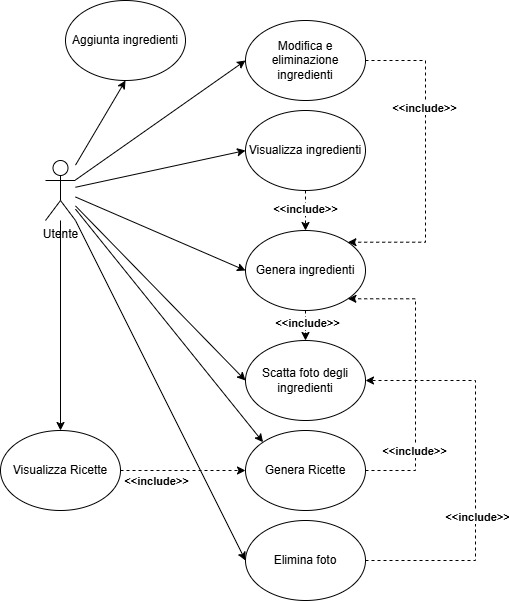
\includegraphics[width=0.8\textwidth,height=\textheight,keepaspectratio]{figures/chapter_1/use_case.jpg}
    \caption{}
    \label{fig:use_case}
\end{figure}

Lo use case in fig.\ref{fig:use_case} mostra lo scenario in cui l'utente ha già aperto entrambe le finestre dell'applicazione, quella per la fotocamera e generazione degli ingredienti e quella per la visualizzazione delle ricette. L'utente potrà scattare una foto ed eliminarla, generare gli ingredienti solo se la foto è stata scattata, aggiungere un ingrediente indipendentemente dalla foto, modificare un ingrediente già presente, generare tre ricette con gli ingredienti presenti e visualizzare le ricette generate.

\section{Architettura}
L'intera applicazione è standalone sul visore, quindi non necessita di un server per il funzionamento. Le uniche operazioni e calcoli che avvengono al di fuori del visore sono quelle che coinvolgono Google Gemini, che avvengono grazie a delle chiamate API in \textbf{POST}.
\section{Interfaccia grafica}
L'interfaccia è composta da due finestre, composte poi da più tabs, e un menu sempre visibile. Ogni finestra ha in alto una barra in cui è presente il nome della finesta e due bottoni posizionati a destra. Il bottone con il simbolo della "X" permette di chiudere la finestra, mentre quello con il simbolo della catena serve a bloccare la finestra nella posizione dove si trova o farsi seguire.
\subsection{Menu}
Il menu che vediamo nella figura \ref{fig:menu} è il menu principale che permette di mostrare e nascondere le finestre dell'applicazione, è composto da tre bottoni e una barra bianca sotto. Andando da sinistra verso destra troviamo il bottone per aprire la finestra per la fotocamera e generazione degli ingredienti, il bottone per vedere le ricette generate e il bottone per fare il pin della barra, in modo da tenerla ancorata nella posizione prefissata. Infatti di default la barra seguirà l'utente posizionandosi in basso in modo da non dar fastidio alle azioni con le altre finestre, sarà possibile spostarla utilizzando la barra bianca in basso.
\begin{figure}[H]
    \centering
    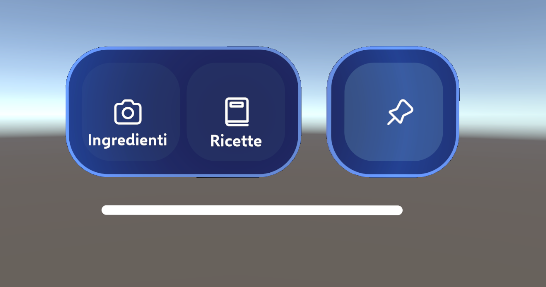
\includegraphics[width=\textwidth,height=\textheight,keepaspectratio]{figures/chapter_1/MENU_interfaccia.png}
    \caption{Menu principale dell'applicazione}
    \label{fig:menu}
\end{figure}
\subsection{Finestra per scatto della foto e generazione degli ingredienti}
Questa finestra è composta da due tabs, una per scattare la foto e visualizzarla come in fig.\ref{fig:camera}, l'altra per visualizzare gli ingredienti generati e apportare modifiche come in fig.\ref{fig:ingredienti}. Per cambiare da una tab all'altra sono presenti due bottoni in alto con in nome "Fotocamera" e "Ingredienti".
\subsubsection{Tab per la fotocamera}
Al centro troviamo la foto scattata, mentre a destra si trova un menu che ci permette di scattare la foto, eliminare la foto già scattata e generare gli ingredienti.
\begin{figure}[H]
    \centering
    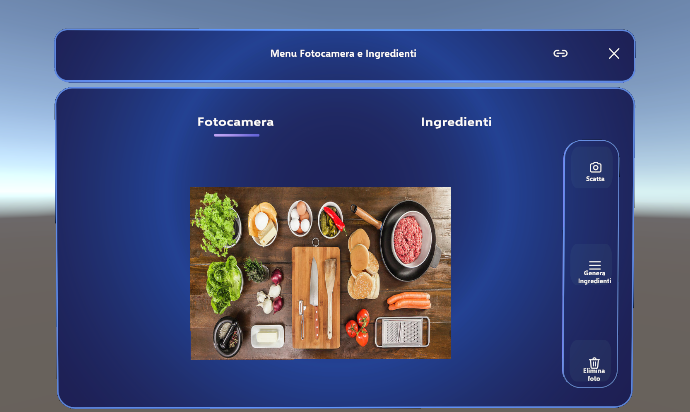
\includegraphics[width=\textwidth,height=\textheight,keepaspectratio]{figures/chapter_1/FOTOCAMERA_interfaccia.png}
    \caption{tab per la visualizzazione e scatto della foto}
    \label{fig:camera}
\end{figure}

\subsubsection{Tab per gli ingredienti}
Nella parte centrale si trova la scroll-list con gli ingredienti, a destra si trova il menu che permette di aggiungere un nuovo ingrediente o creare tre ricette con gli ingredienti presenti. Per la modifica di un ingrediente è necessario cliccare su di esso nella lista, in questo modo si aprirà una finestra di modifica come in fig.\ref{fig:modifica}.

\begin{figure}[H]
    \centering
    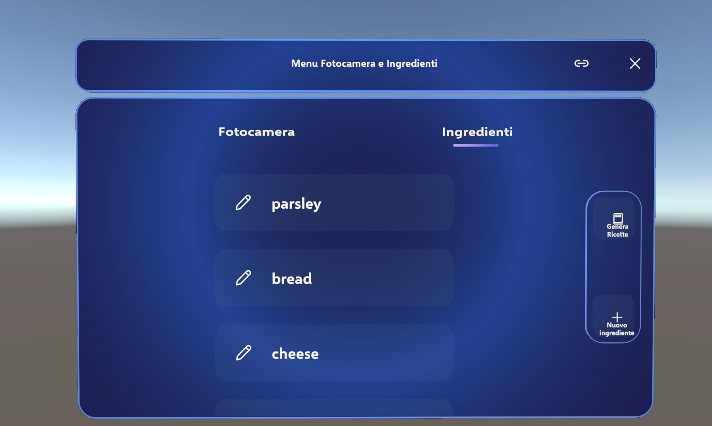
\includegraphics[width=\textwidth,height=\textheight,keepaspectratio]{figures/chapter_1/INGREDIENTI_interfaccia.png}
    \caption{Tab per la visualizzazione, inserimento  e modifica degli ingredienti}
    \label{fig:ingredienti}
\end{figure}

\begin{figure}[H]
    \centering
    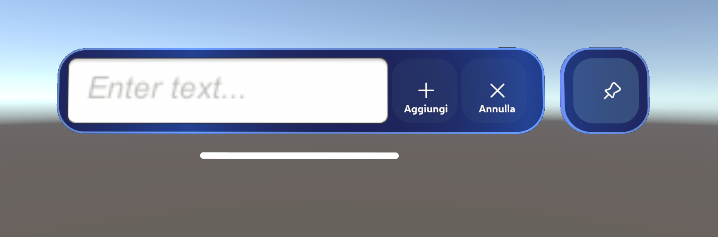
\includegraphics[width=\textwidth,height=\textheight,keepaspectratio]{figures/chapter_1/AGGIUNGI_interfaccia.png}
    \caption{Aggiunta di un ingrediente}
    \label{fig:aggiunta}
\end{figure}

\begin{figure}[H]
    \centering
    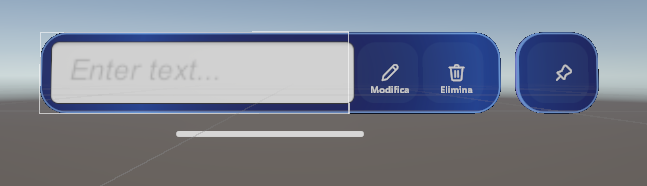
\includegraphics[width=\textwidth,height=\textheight,keepaspectratio]{figures/chapter_1/MODIFICA_interfaccia.png}
    \caption{Modifica di un ingrediente}
    \label{fig:modifica}
\end{figure}




\subsection{Finestra per visualizzazione delle ricette}
In alto troviamo un menu con tre bottoni che ci permettono di cambiare tab, ogni tab è composta da una scroll-list con le ricette generate. A destra troviamo un bottone che permette di generare nuove ricette.

\begin{figure}[H]
    \centering
    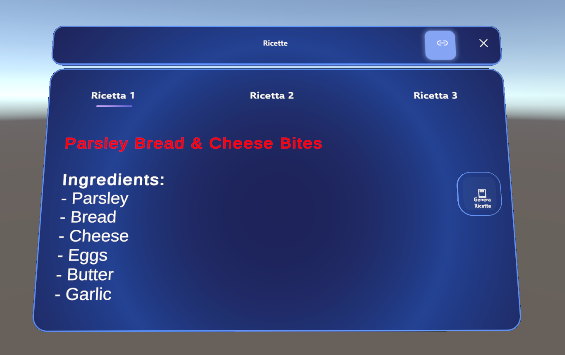
\includegraphics[width=\textwidth,height=\textheight,keepaspectratio]{figures/chapter_1/RICETTE_interfaccia.png}
    \caption{Interfaccia per la visualizzazione delle tre ricette}
    \label{fig:ricette}
\end{figure}



\section{Persistenza dei dati}
I dati vengono salvati in due file JSON, uno che contiene gli ingredienti e l'altro le ricette generate, la foto scattata invece viene salvata nella stessa direcory dei file JSON sotto un nome specifico. I nomi dei file si trovano all'interno di un file config, nella cartella StreamingAssets,  accessibile e leggibile come indicato in fig.\ref{fig:streamingAssets}

\begin{figure}[H]
    \centering
    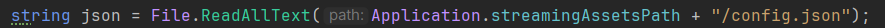
\includegraphics[width=\textwidth,height=\textheight,keepaspectratio]{figures/chapter_1/streamingAssets_CODICE.png}
    \caption{Codice per leggere il file di config}
    \label{fig:streamingAssets}
\end{figure}

Successivamente, grazie alla classe generica \textbf{FileHandler} possiamo serializzare e deserializzare i file JSON salvati, per modificarli o crearli. 
I file JSON  e l'immagine vengono salvati nel \textbf{persistentDataPath} come indicato in fig.\ref{fig:persistentDataPath}.

\begin{figure}[H]
    \centering
    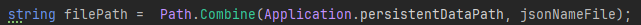
\includegraphics[width=\textwidth,height=\textheight,keepaspectratio]{figures/chapter_1/persistentDatapath_CODICE.png}
    \caption{Parte di codice che genera il path in cui salvare il file JSON}
    \label{fig:persistentDataPath}
\end{figure}